\subsection{Flight Tests}
\label{sec:diary}
The Gantt chart cannot fully express the amount of ongoing testing (including flight tests) and iterative design that was performed every week of each semester. Table \ref{tab:tests} documents all major external tests and pre-flight checks performed on the Dragonfly (Prototype \#2) aircraft throughout the year; for brevity, there are a large number of minor tests that are not included in the table. 

\begin{table}[H]
	\centering
	\caption{Flight tests performed by \ID}
	\begin{tabular}{|c|c|c|c|c|c|c|}
		\hline Date & Location & Flight Time & Aim & Result & Problems \\
		\hline 02/07/15 & Melb Uni & 2 min & Courtyard Alt-Hold test & Complete & - \\ 
		\hline 03/07/15 & Cardinia & 15 min & Major test/Autotune & Complete & Radio cut outs \\ 
		\hline 27/07/15 & Cardinia  & 0 min & Autotune new firmware & Incomplete & Radio faillure \\ 
		\hline 31/07/15 & Cardinia  & 6 min & Autotune new firmware & Crash & Motor burnt out, damage  \\ 
		\hline 22/08/15 & Cardinia  & 2 min & Autotune new firmware & Crash & Power Module Failure, damage\\
		\hline 04/09/15 & Melb Uni & 1 min & Courtyard Alt-Hold test & Complete & - \\  
		\hline 05/09/15 & Cardinia  & 8 min & Autotune new firmware & Complete & Back gear broken\\
		\hline 18/07/15 & Melb Uni & 1 min & Courtyard Alt-Hold test & Complete & - \\  
		\hline 19/09/15 & Cardinia  & 10 min & Test flight with wings & Complete & Overheating \\ 
		\hline 27/09/15 & Cardinia  & 5 min & Test transition & Incomplete & Solder melting (overheating) \\
		\hline 04/10/15 & Cardinia & 3 min & Test transition & Incomplete & Too windy\\
		\hline 
	\end{tabular} 
	\label{tab:tests}
\end{table}

\subsection{Project Diary}
The team has made extensive use of Trello to maintain records of the tasks performed throughout the project. The project's records/diary may be viewed in full detail here: \url{https://trello.com/uavoutbackchallenge2016}.

\subsection{Project Timeline}
\subsubsection*{Gantt Chart}
\label{sec:gantt}
See Figure \ref{fig:gantt} for a detailed development timeline for this project, including additional tasks from Progress Report \#1 (highlighted in orange), removed tasks (crossed out) and incomplete tasks (highlighted in red). 

\subsubsection*{Major Problems and Issues}
Throughout the year, there were a number of problems that significantly delayed the progress of the project. The Gantt chart provides some details regarding the time delay as a result of each problem.
\begin{itemize}
	\item Vibrations and stability: In semester 1, more time than initially planned was spent on eliminating vibrations and increasing stability of the aircraft. 
	
	\item Printer repair: Many hours have been spent fixing and tweaking the 3D printer.  During the holidays, a week of testing and repair was done to fix an issue with clogged nozzles (listed as "Reparing 3D printer problems" in the Gantt chart). 
	
	\item Multiple crashes: Crashes throughout the year required the purchase of replacements parts, and corresponding delays due to shipping time. Large amounts of time were then spent repairing an=d re-testing components (listed as "Modifications and repairing aircraft problems" in the Gantt chart). All major crashes were due to faulty hardware such as the power module, RC transceiver and failure of a motor, resulting in the fixed-wing flight controller not being fully tested. As such, a final version of an autonomous fixed wing flight controller could not be implemented (listed as "Confiure automated flight controller for fixed wing" in the Gantt chart), and thorough testing of the hybrid aircraft's capabilities could not be completed. 
	
	\item Team Member Departure: As a result of family issues, Shanon was unable to make meaningful contributions after semester 1 (including mid year break), particularly during the final weeks before the submission of final report. Several sections of the Gantt chart (his tasks) remain incomplete as a result of this.
\end{itemize}

\subsection{Scope of Works}
See below for the final version of team \ID Scope of Works.

\begin{landscape}
\vspace*{20pt}
\begin{figure}[!ht]
	\centering
	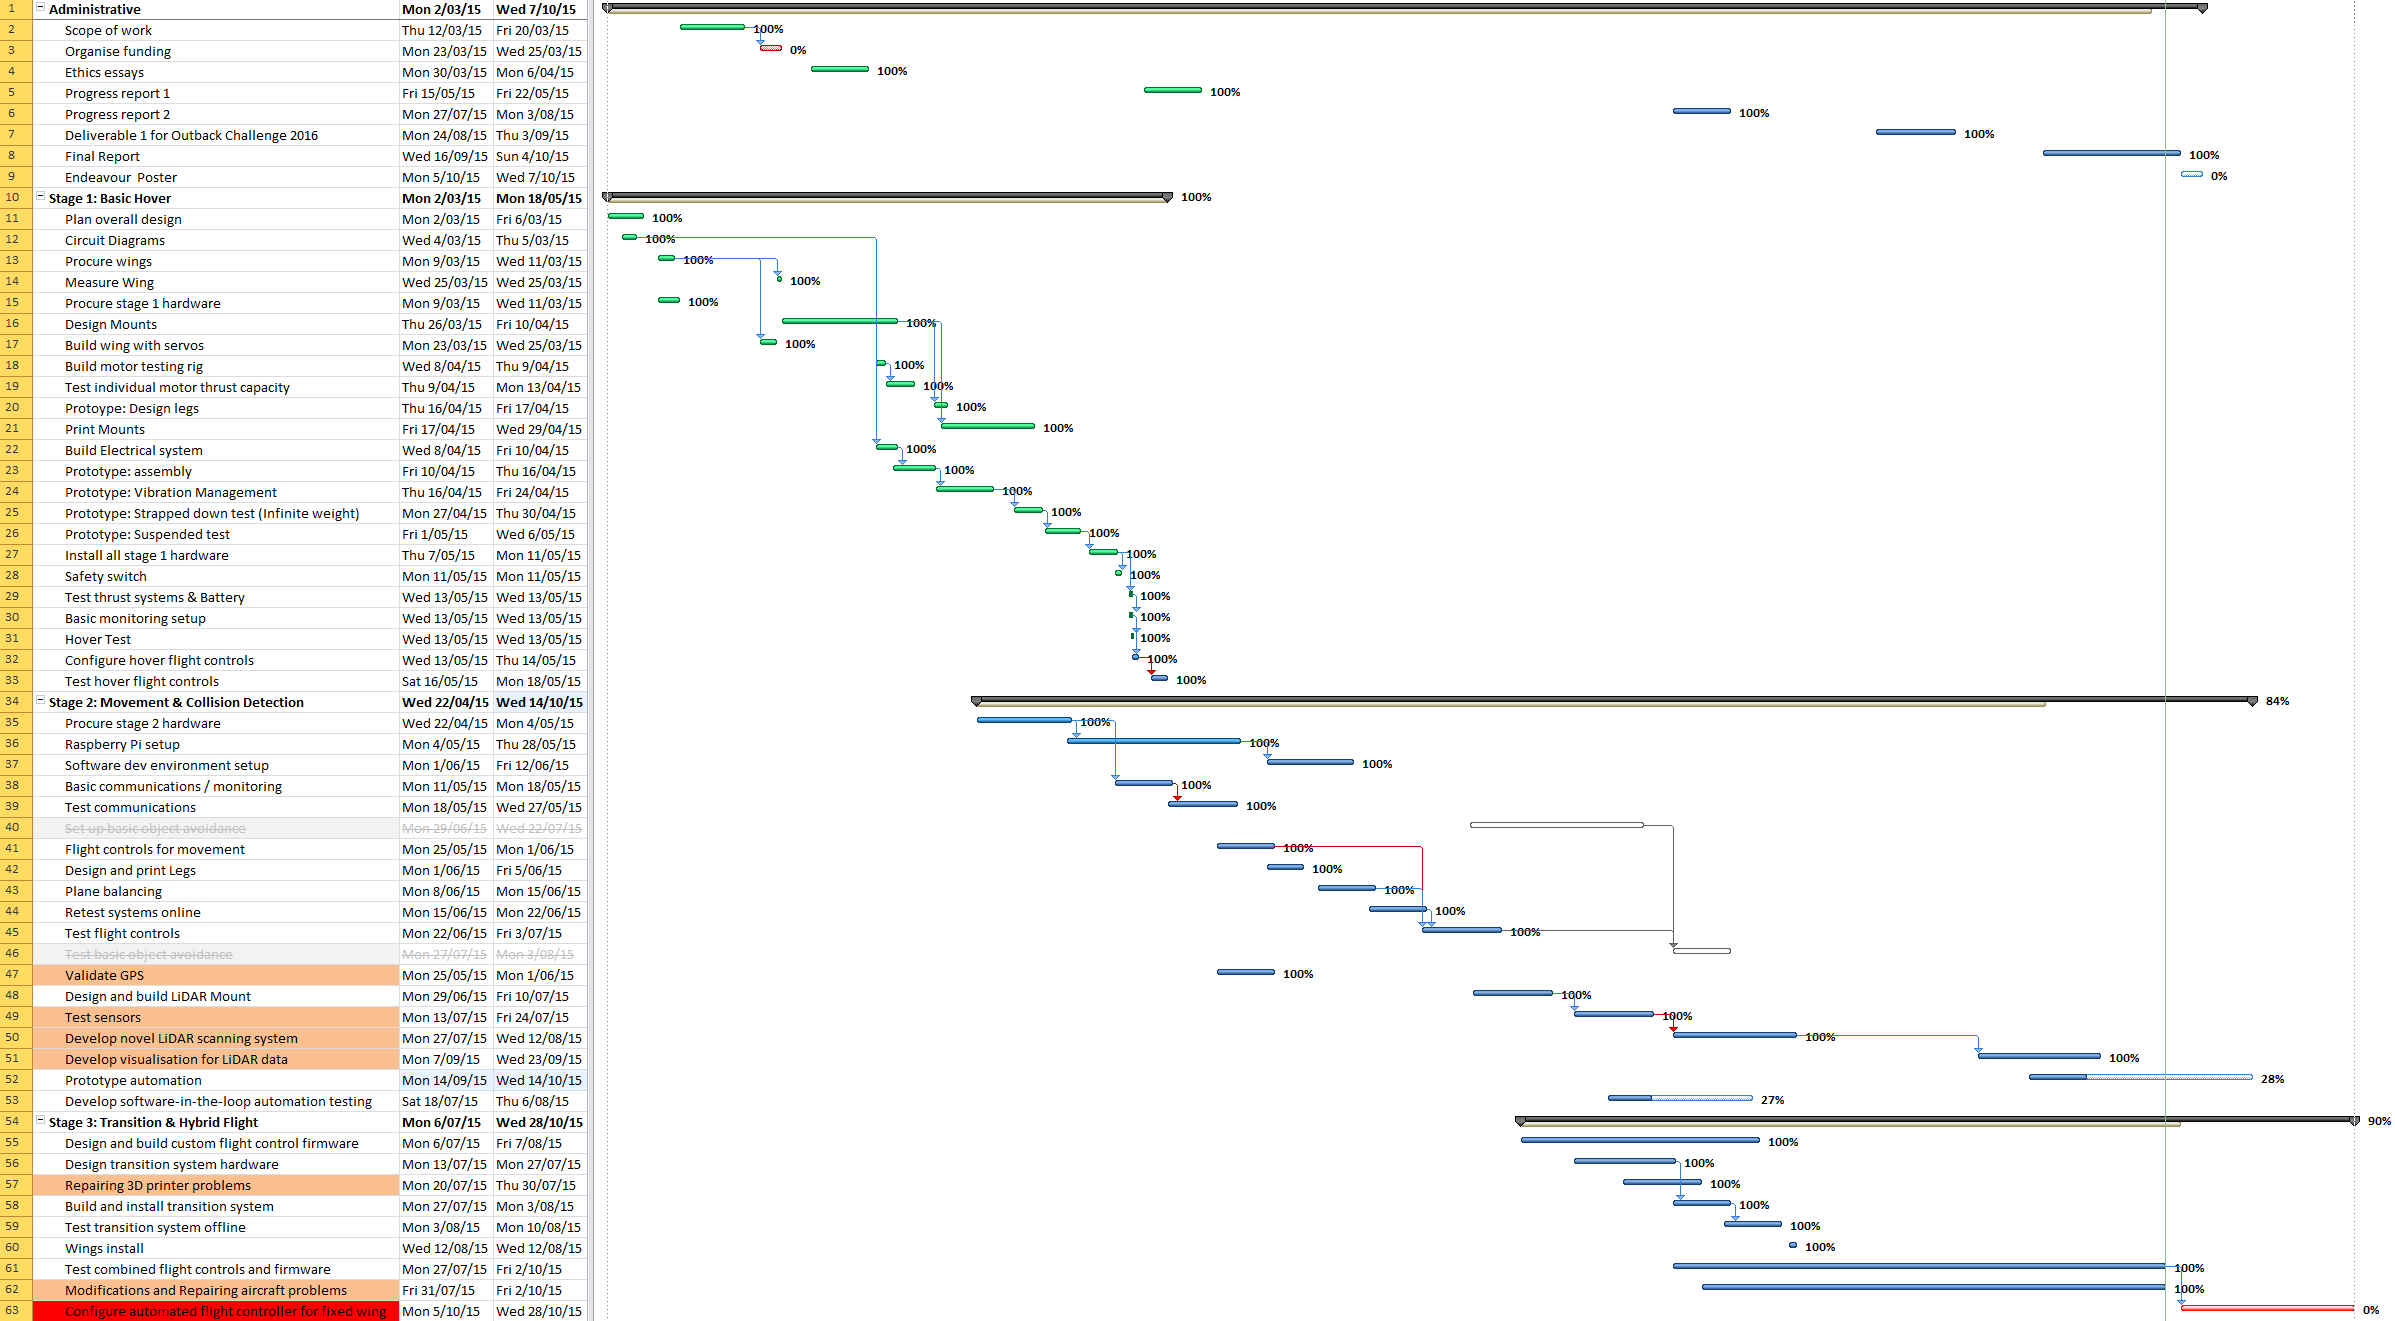
\includegraphics[width=730pt]{\IMAGEPATH /Diagrams/gantt}
	\caption{\ID Gantt Chart}
	\label{fig:gantt}
\end{figure}
\end{landscape}

\iffinal

\includepdf[pages=2-]{scope.pdf}
\fi